\chapter{Machine Learning for Tracker Data Quality Monitoring (ML4DQM) \label{ch:DQM}}

\section{DQM Workflows}

Physicists at CMS use the world’s largest and most complex machinery to probe the fundamental forces of nature. An overwhelming amount of new data collected poses a challenge for its processing and storage. This necessitates designing algorithms and special software to control the data quality. The process of monitoring the data flow from the CMS detector and certifying for physics analysis is referred to as Data Quality Monitoring (DQM). A quick online feedback on the quality of the data recorded is essential to collect high-quality data and guarantee a good baseline for the offline analysis.


Datasets from the collisions that are certified as "Good" by the DQM process are critical towards the search for physics Beyond the Standard  Model and to look for any new signs of discoveries. Hence, DQM plays a important role in assessing the health of the detector elements, its operation efficiency, and performs reliable data certification\cite{refId0}.

%Physicists at CERN use the world’s largest and most complex machinery to probe the fundamental forces of nature. The idea of Data Quality Monitoring (DQM) is simple, monitor the data flow from the Compact Muon Solenoid (CMS) detector and certify that it is useful for physics analysis. To operate a sophisticated and complex apparatus as CMS, quick online feedback on the quality of the data recorded is essential to collect high-quality data and to guarantee a good baseline for the offline analysis. Collecting good datasets from collisions and certified by the DQM process is a critical step towards the search for ``new physics". As an overwhelming amount of new data poses an extra challenge of processing and storage this makes it all the more important to design algorithms and special software to control the data quality. Hence, DQM plays a critical role in the maintainability of the experiment, the operation efficiency, and it also performs reliable data certification\cite{refId0}.


The current paradigm (see \Cref{fig:DQM_workflow}) of DQM has the human shifter in mind. A person spends hours looking at various histograms that indicate the status of the data flow, detector conditions, and other activities. These histograms are checked manually and visually against a reference to help determine the data quality and detector performance.
\begin{figure}
	\centering
	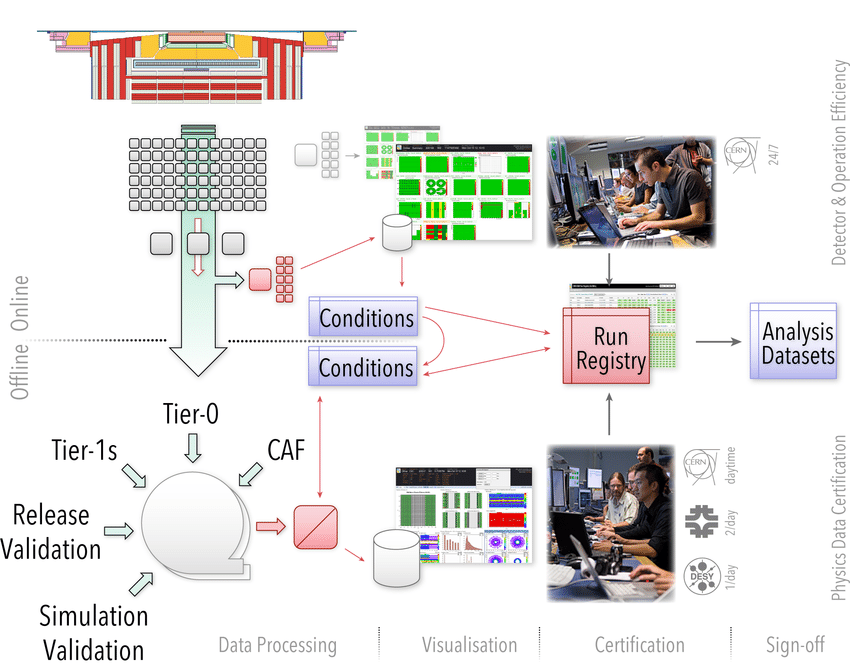
\includegraphics[width=.89\linewidth]{Images/DQM Workflow.png}
	\caption{The DQM workflow}
	\label{fig:DQM_workflow}
\end{figure}
The DQM workflow consists of 2 types: Online and Offline.
The Online DQM consists of receiving data taken from the event and trigger histograms to produce results in the form of monitoring elements like histogram references and quality reports. This live monitoring of each detector’s status during data taking gives the online crew the possibility to identify problems with extremely low latency, minimizing the amount of data that would otherwise be unsuitable for physics analysis. The scrutiny of the Online DQM is a 24/7 job that consists of shifters that work at the CMS control center constantly monitoring the hundreds of different plots and histograms produced by the DQM software. This consumes a lot of manpower and is strenuous work.
Offline DQM is more focused on the full statistics over the entire run of the experiment and works with bookkeeping and data certification. In the offline environment, the system is used to review the results of the final data reconstruction on a run-by-run basis, serving as the foundation for certified data used across the CMS collaboration in all physics analyses.


\section{DQM Tools}
The DQM tools allow shifters to gather the information necessary for performing data certification. The platform used to certify any run's worth of data is the \textit{Certification Helper} (see \Cref{fig:certhelper}). This is a web application that provides shifters with information about the runs that have or have not been certified.
Inside this tool, one can view (as shown in \Cref{fig:certhelper-portal,fig:certhelper-cert}) the list of runs certified, a portal to select runs for certification, and a page with a checklist to certify the run.

\begin{figure}
	\centering
	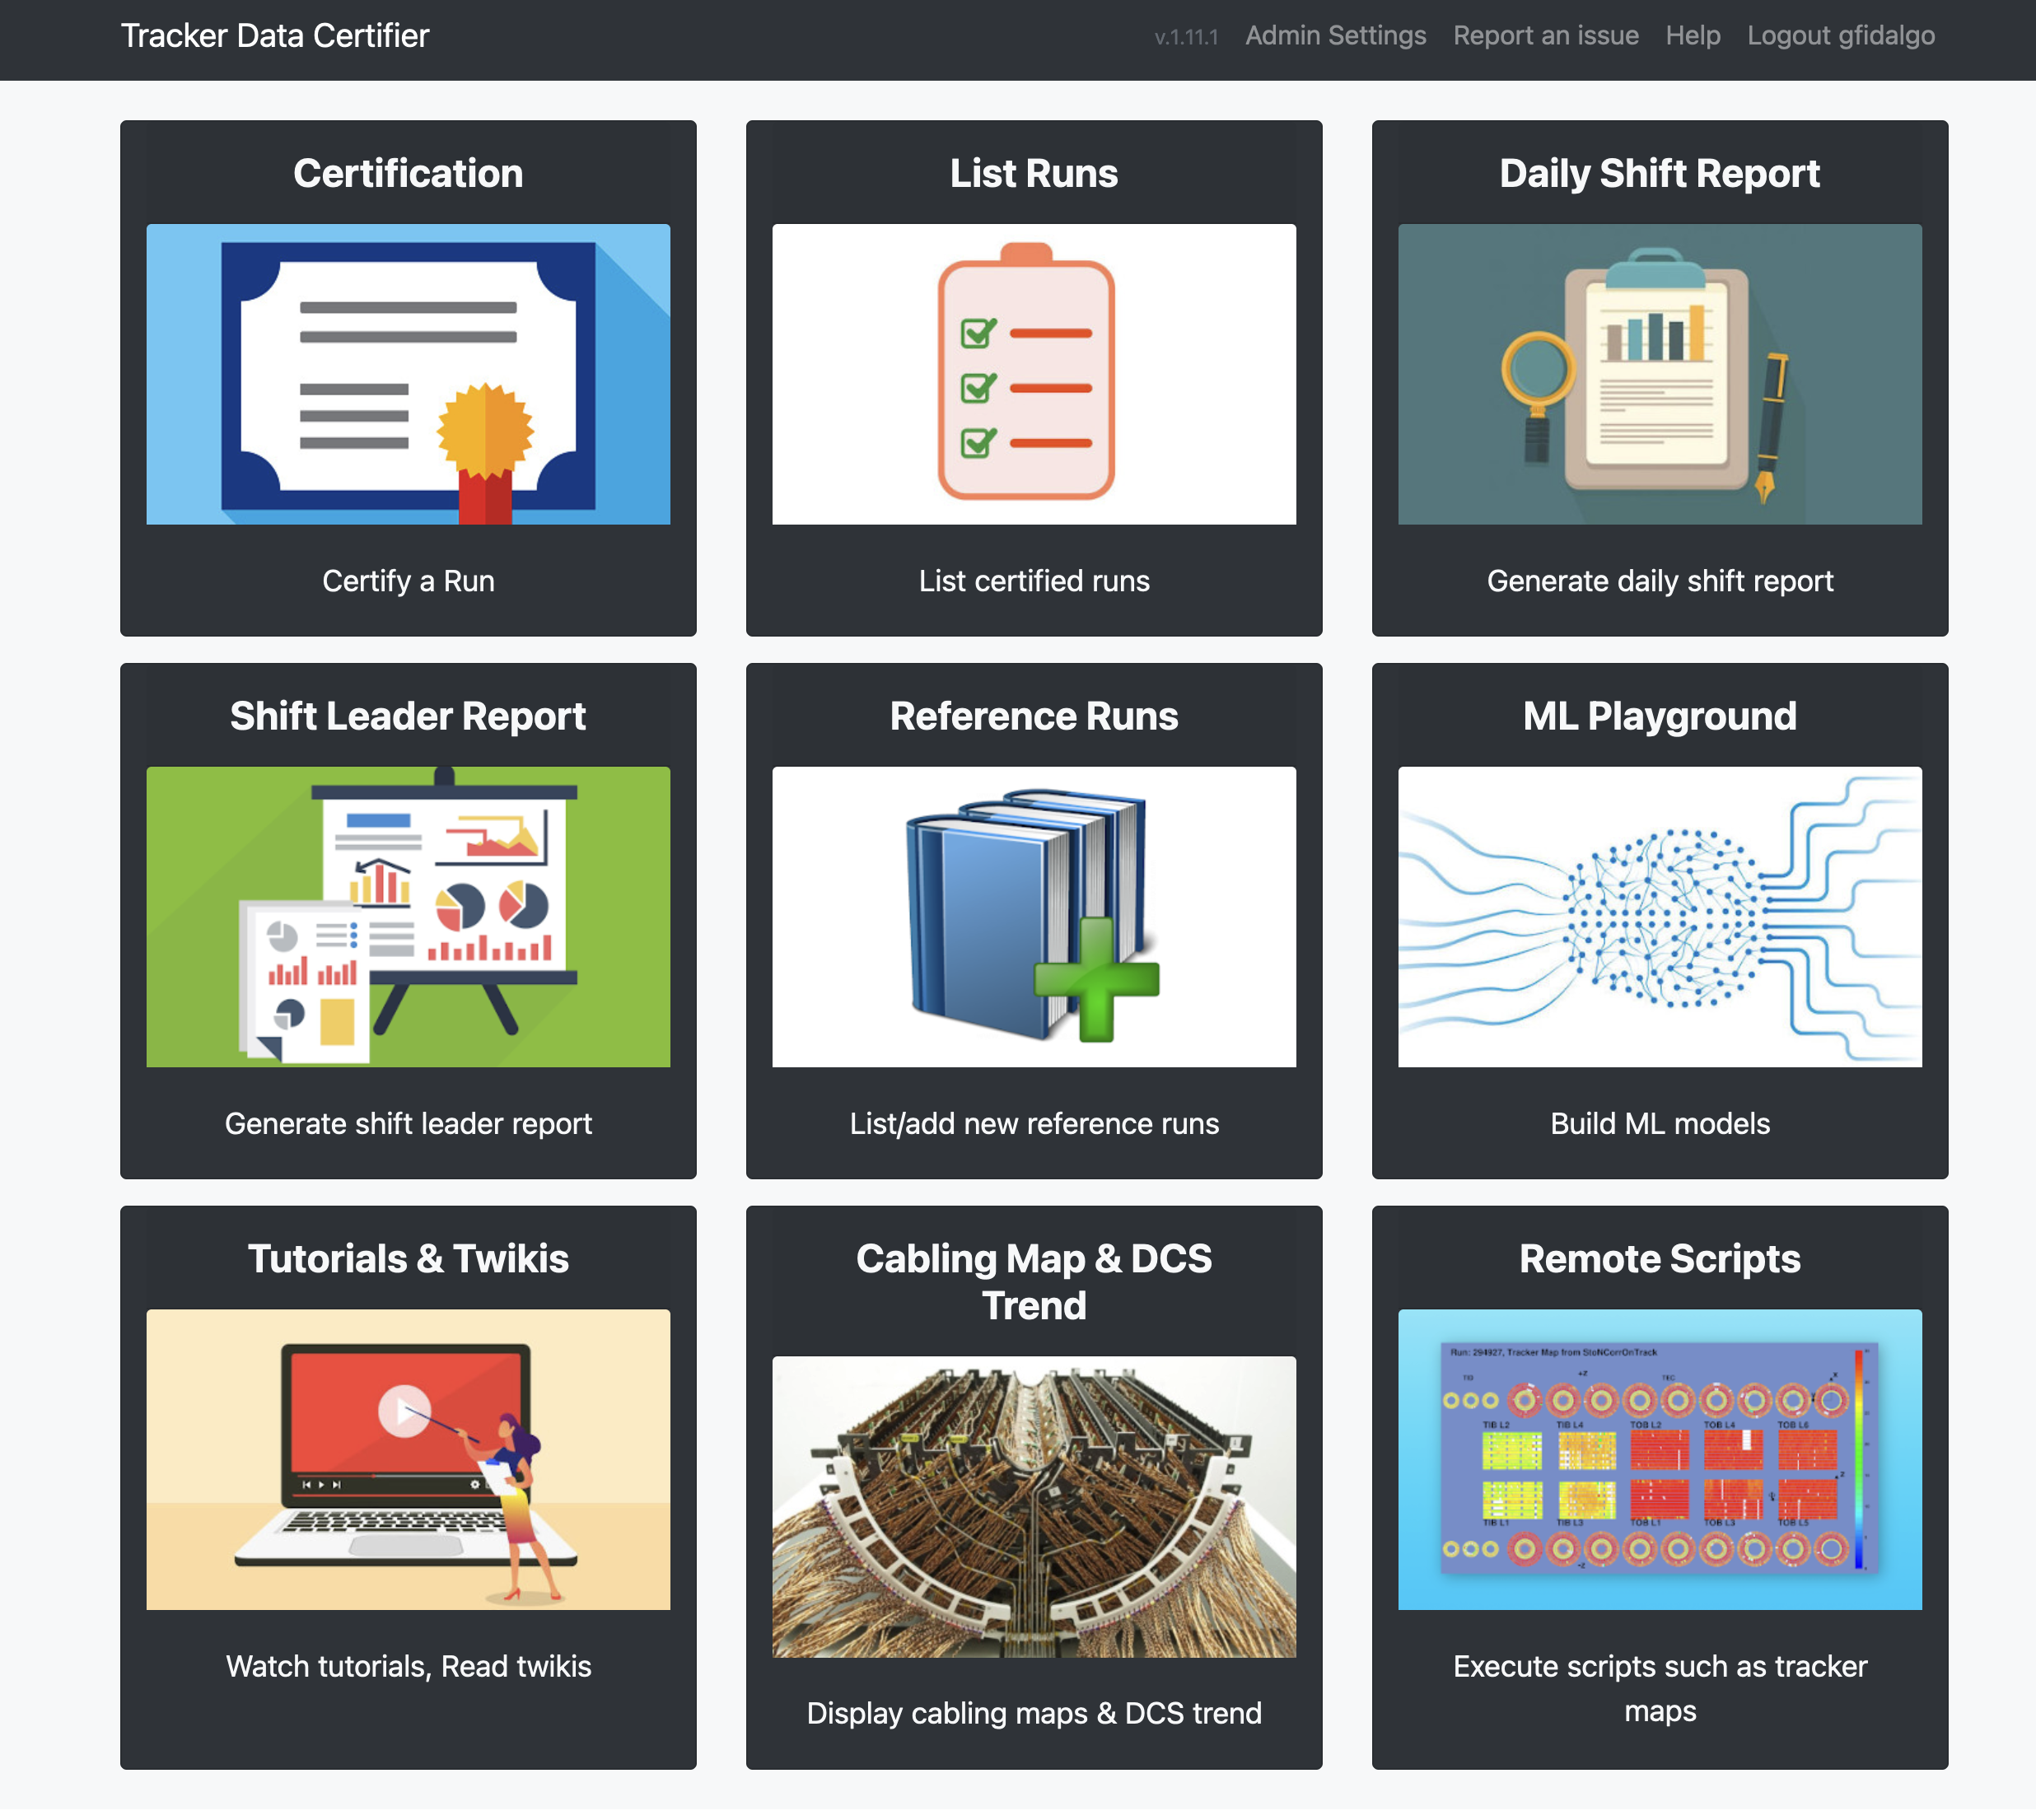
\includegraphics[width=.75\linewidth]{Images/certhelper-menu.png}
	\caption{\textit{Certification Helper} is a web app that allows shifters to view, certify, and gather information on a given run.}
	\label{fig:certhelper}
\end{figure}

\begin{figure}
	\centering

	\begin{subfigure}{.7\linewidth}
		\includegraphics*[width=\linewidth,trim= 4in 1.5in 4in 0]{Images/certhelper-portal.png}
	\end{subfigure}

	\begin{subfigure}{\linewidth}
		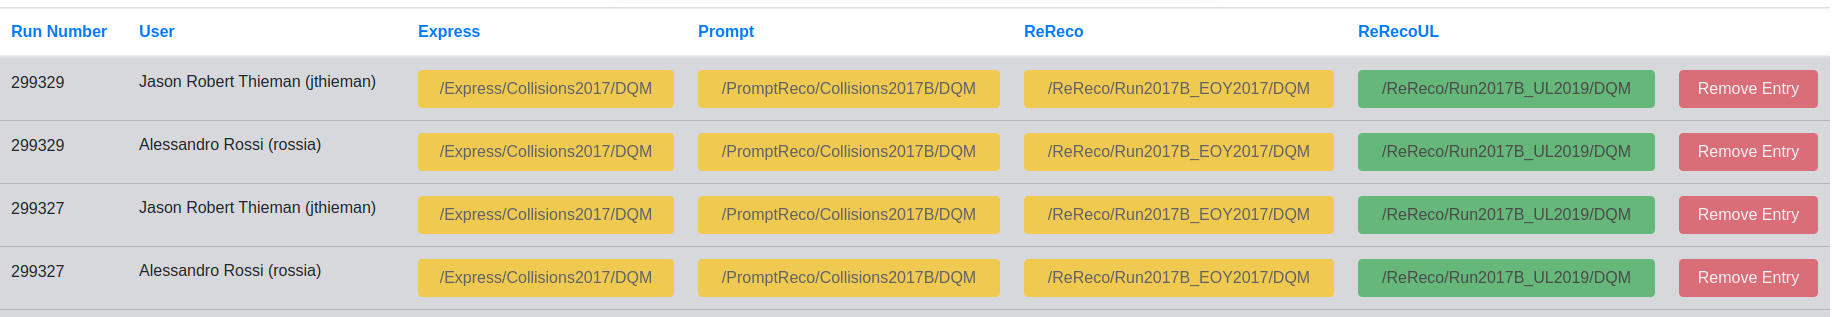
\includegraphics[width=1\linewidth]{Images/certhelper-list.png}
	\end{subfigure}
	\caption{The \textit{Certification Helper} portal that allows shifters to select and view which runs are available to certify.}
	\label{fig:certhelper-portal}
\end{figure}
\begin{figure}
	\centering
	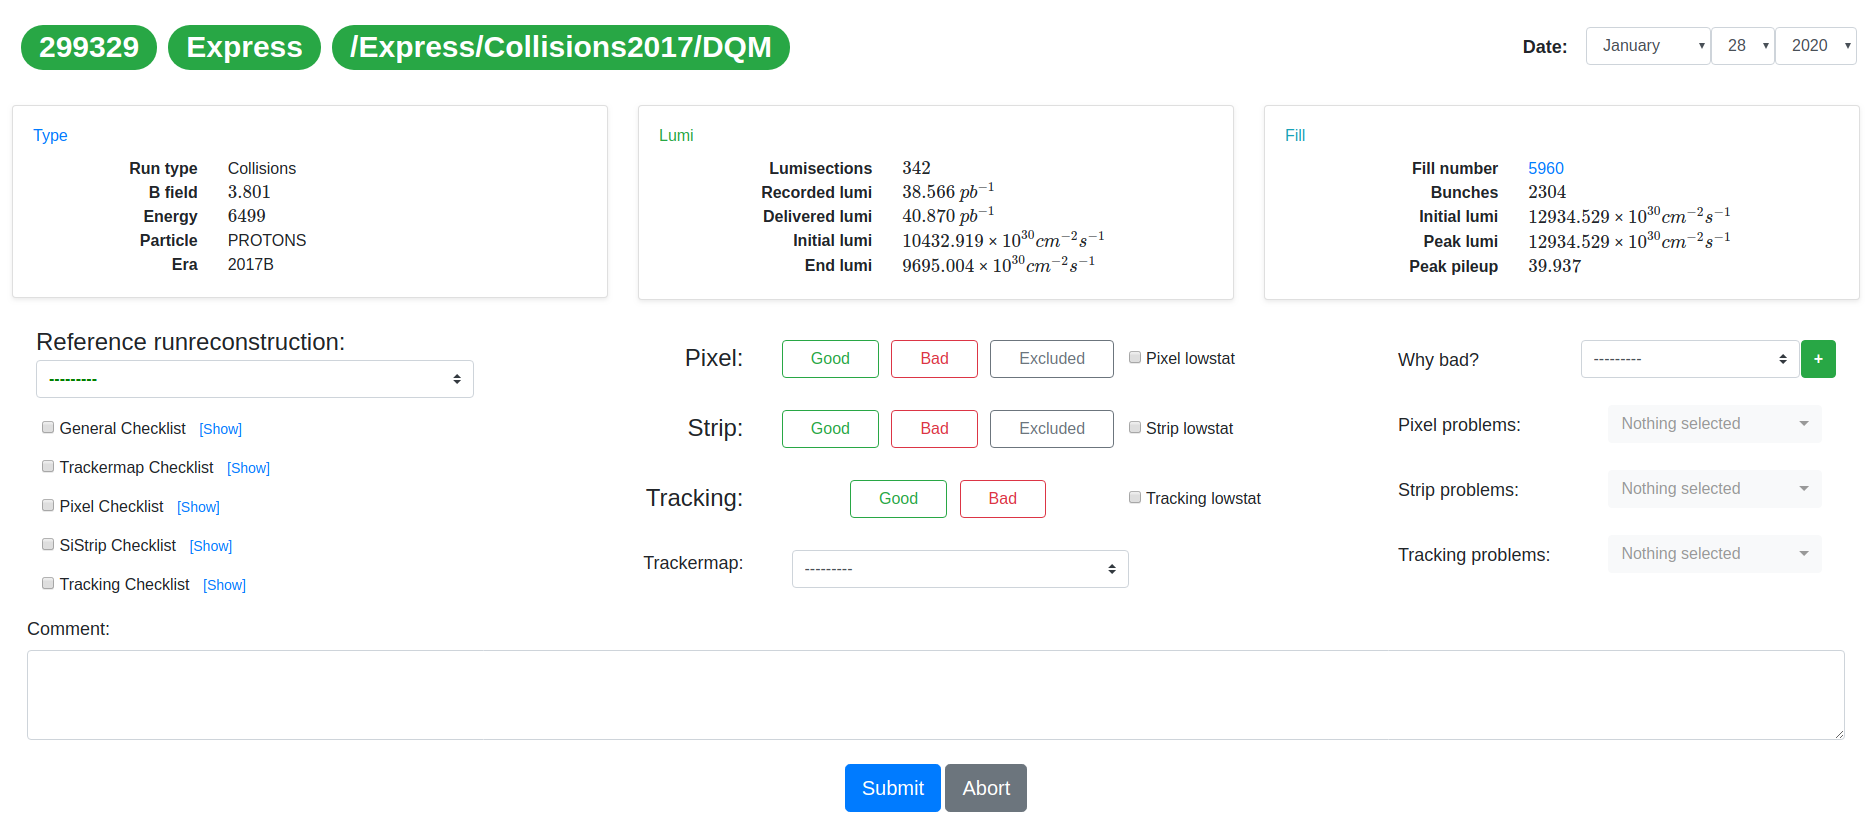
\includegraphics[width=1\linewidth]{Images/certhelp-cert.png}
	\caption{The view when certifying a run on \textit{Certification Helper}}
	\label{fig:certhelper-cert}
\end{figure}


Other DQM tools that are frequently used are the \textit{DQM GUI}, \textit{Run Registry}, and \textit{Online Monitoring System} (OMS). We can see snippets of those tools in \Cref{fig:dqmgui,fig:RR,fig:OMS}.


\begin{figure}
	\includegraphics*[width=\linewidth,trim= 0 7in 1in 0 ]{Images/DQM GUI.png}
	\caption{The DQM GUI shows many histograms that shifters use to determine the quality of a run.}
	\label{fig:dqmgui}
\end{figure}

\begin{figure}
	\includegraphics*[width=\linewidth,trim= 2.9in 4.4in 0 0in]{Images/RR.png}
	\caption{Run Registry. This page is a database that shows the datasets where each run is classified to and also shows it's DQM certification.}
	\label{fig:RR}
\end{figure}


\begin{figure}
	\includegraphics*[width=1\linewidth,trim = .8in 1.1in .9in 2.19in]{Images/OMS.png}
	\caption{OMS webpage. This shows detector and data taking conditions and statistics}
	\label{fig:OMS}
\end{figure}


\section{Challenges of DQM}

The current DQM process presents many challenges that need to be addressed:
\begin{itemize}
	\item The process ultimately depends on the decisions made during DQM shifts. As time passes shifters must be trained regularly to learn the DQM process and each particular subsystem's specific metrics. The dependence of human shifters leaves the process vulnerable to unforeseen outside influences (such as getting sick, a pandemic, lack of worker availability, etc.). This allows for unpredictable mistakes and biases in the monitoring and certification workflows.

	\item  Worsening this, the amount of histograms to be checked is on the order of 50-100 per hour and many have unique metrics to define what is considered nominal. People can make mistakes and miss errors even with a dedicated team of experts for each subsystem to guide the shifters.

	\item The detector is subject to transient problems that can be overlooked during visual inspection of the monitoring elements. \cite{ML4DQM}

	\item Detector conditions can change drastically enough to require a change in the selection of the reference material. Shift experts also determine this.

	\item A lot of documentation can be found to learn about the DQM procedure. But again, this needs to be kept up-to-date manually. Sometimes these can be outdated, affecting shifter decisions.

	\item The current workflow certifies data on a run-by-run basis (i.e. run granularity). This is especially relevant with the upcoming HL-LHC, where detector conditions will allow for more data to be collected per unit of time.
\end{itemize}

To address some of these issues, recent campaigns have emerged to reduce the manpower that both Online and Offline DQM entail. With the development of Machine Learning techniques, the hope is to automate the DQM scrutiny to a point where shifters can give better quality certifications more efficiently. We also desire to use ML to sift through data with more time using shorter time intervals known as the luminosity section (LS) granularity.
Each run is divided into LSs, an interval corresponding to a fixed number of proton-beam orbits in the LHC and amounting to approximately 23 seconds.
This finer granularity increases the number of histograms to be monitored by 1 or 2 orders of magnitude, making it unfeasible for human certification\cite{ML4DQM}. The work presented here tries to follow in this direction in order to help improve the effort.

\section{Reference Run Ranking (non-ML)}

% The project aimed to develop a ranking system for identifying reference runs used in ML-enabled DQM workflows. Reference runs are chosen based on their data-taking conditions, statistical robustness, and similarity to the target run. Currently, an expert shifter decides when a new run should be considered as a reference based on these criteria. The ultimate decision is made by the shift leader.

To enable tools for machine learning-enabled Data Quality Monitoring (DQM) workflows, a project was undertaken to develop a ranking system for runs to be used as references. Reference runs are typically considered nominal due to the data-taking conditions present in them. Additionally, a reference run must be long enough (i.e. have many LSs) to provide meaningful statistics. Currently, the decision of whether a new run should be considered as a reference is made by an expert shifter based on data-taking conditions and feedback from DQM shifters. The candidate reference run must pass several quality checks, including containing a high number of LSs to ensure statistical robustness and having data-taking conditions as similar as possible to the target run.
Ultimately, the shift leader decides if a run becomes the next reference. This system aims to simplify reference run selection and provide shifters with high-quality runs for ML model training accessible through the \textit{Machine Learning Playground} (more on \Cref{sect:MLP}). I have initiated work on a ranking system that will present shift leaders with a table of potential candidates. This system will rank the candidate runs from best to worst based on their suitability as reference runs. It will consider factors such as run length, age, and the number of pileup collisions per event. These comparisons will be graded and the results presented in a table as seen in \Cref{fig:ranking}.
% The ranking system will provide shift leaders with a table of potential reference run candidates ranked from best to worst based on their suitability and quality. It takes into account factors such as run length, age, and number of pileup collisions per event. This will make it easier to identify high-quality runs and provide robust training datasets for ML models accessible through the MLP.
Past efforts failed to consistently place the reference run at the top of the list of candidates due to two main problems: firstly, the parameters characterizing each run were not normalized, leading to an artificial inflation of the importance of some parameters over others and secondly, the weights assigned to each parameter were not systematically determined but were instead based on expert opinion and experience.
Weighted Euclidean distance between the feature vectors of the candidate runs and the target run would be computed to gauge the similarity between the target run and the reference candidates. In the future, a systematic approach will be implemented to determine the appropriate weights for this metric, which will include the normalization and possible standardization of features to ensure that they are comparable irrespective of the statistical approach chosen.


\begin{figure}
	\centering
	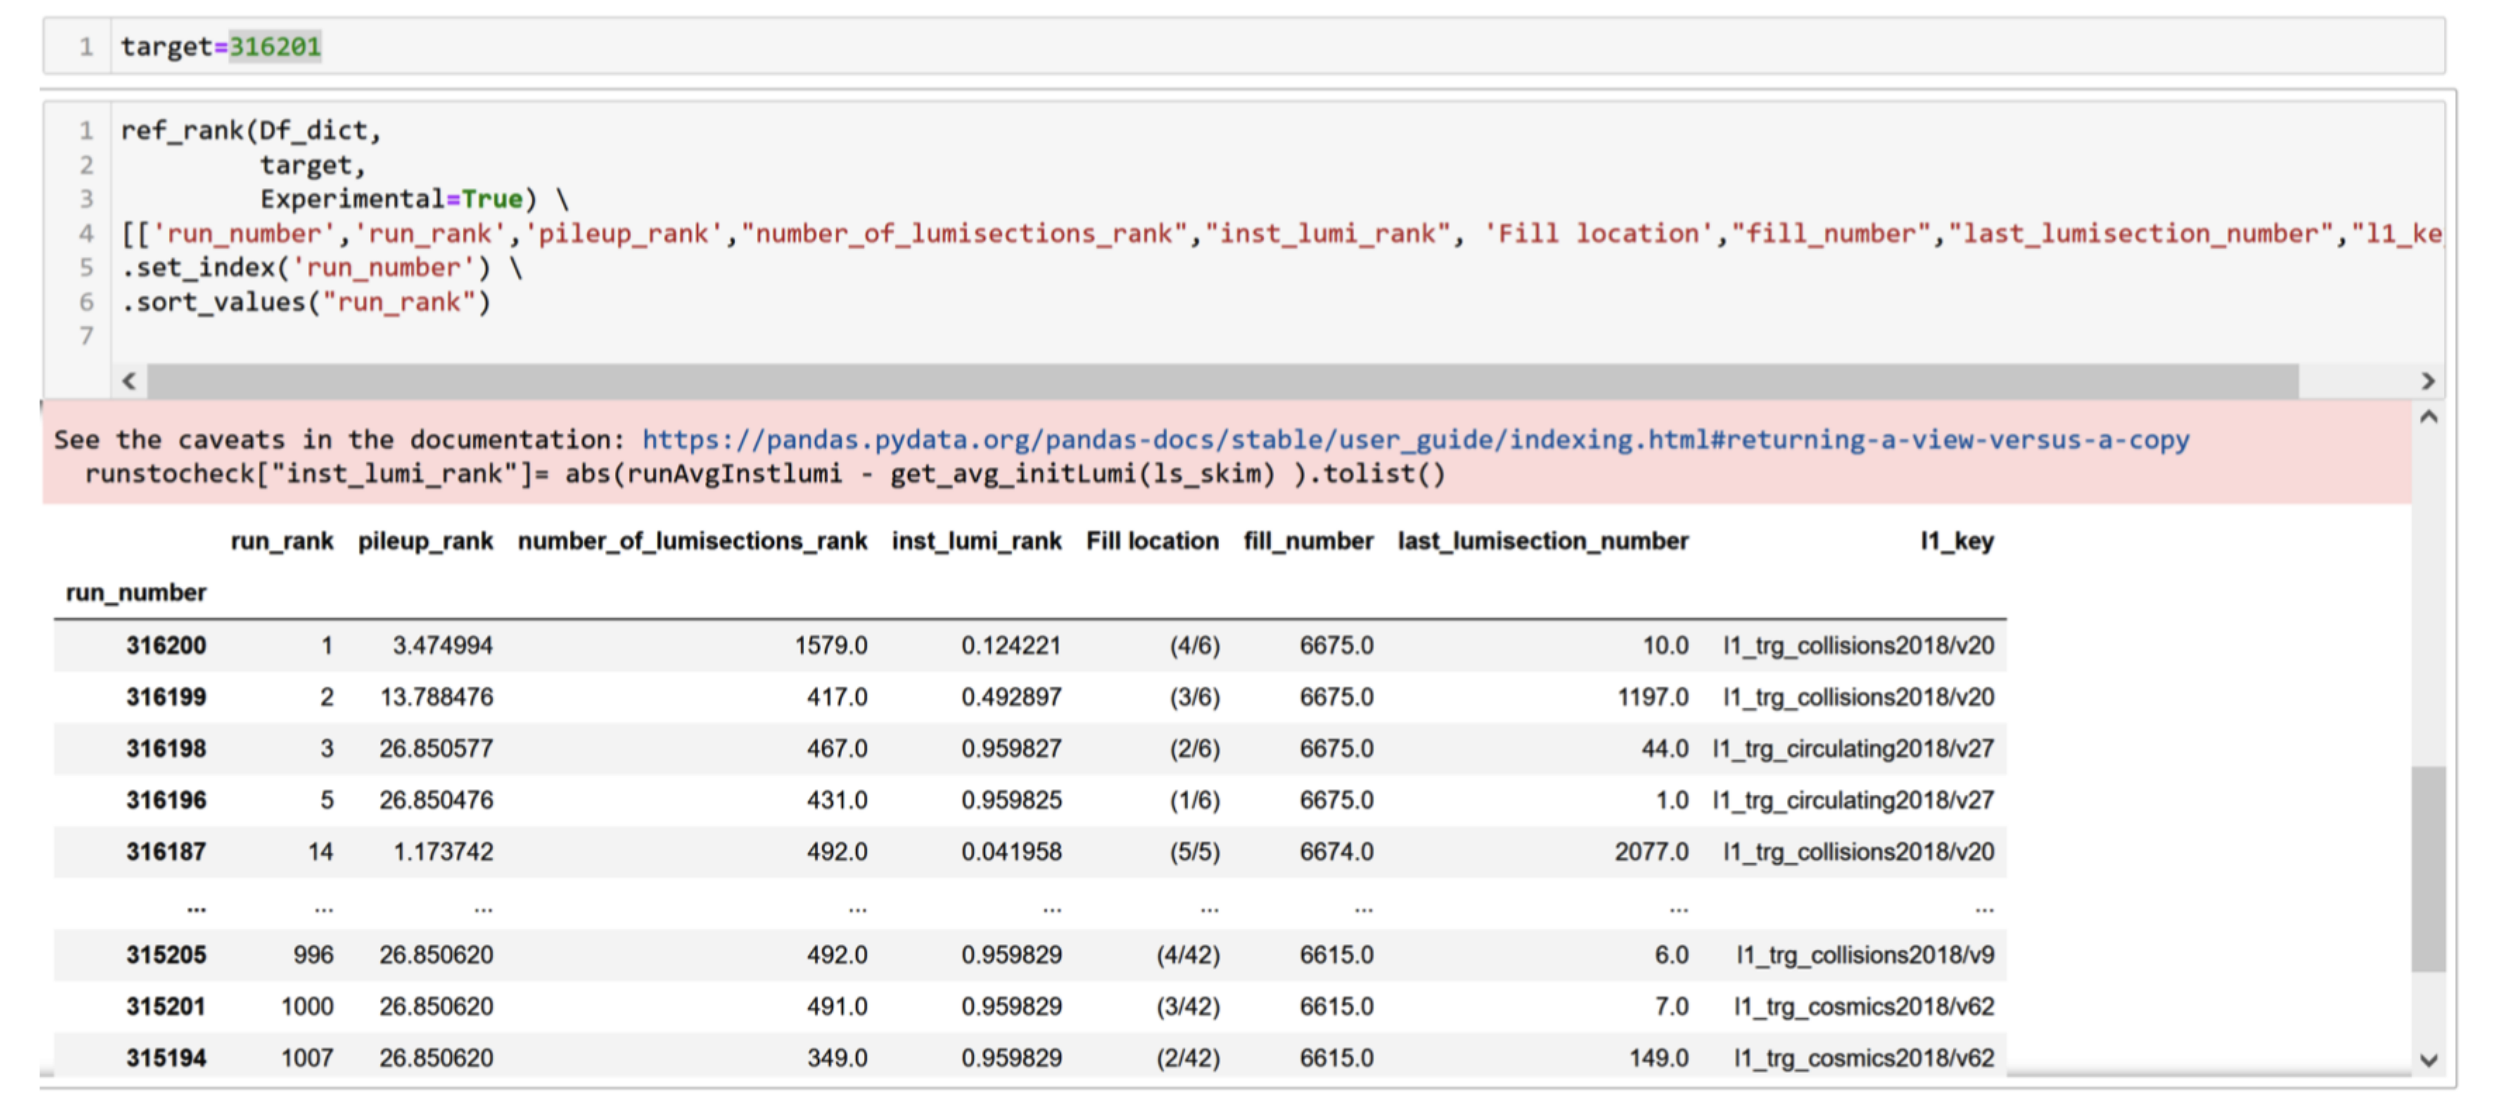
\includegraphics[width=\linewidth]{Images/ranking.png}
	\caption{Reference run ranking system demo.}
	\label{fig:ranking}
\end{figure}


\section{ML Playground}\label{sect:MLP}
Following the spirit to move towards an ML-enabled DQM, an effort to develop a platform where ML models can be deployed, trained, and tested for data certification has resulted in what is now called the \textit{Machine Learning Playground} (MLP). MLP is a Django-based framework, to automate DQM\cite{Wachirapusitan_2023}. It groups training dataset information, automates ML training, and generates reports based on the performance of an ML model. It is a web application that provides easy access to the most common monitoring elements that are found in the DQM GUI, as well as the data-taking conditions and information found in OMS and the RunRegistry. It allows for simpler data exploration when interacting with it through its Python API. It is designed to be scalable, allowing users of other subsystems to benefit from the playground by hosting all the necessary subsystem-specific information.

In this project, I developed code to automate the data ingestion of the MLP by using a cronjob. This cronjob executes a query from another database called \textit{Data Aggregation System} (DAS), to gather lists of newly generated files continuously. The script later downloads and copies files to our CERN-based filesystem called EOS. Afterward, the script will index the newly copied files to the MLP database and execute the MLP's parsing capabilities, allowing the MLP to read and portray the information contained inside the files.
I have added logging functionality for detailed bookkeeping in case the scripts involved fail.


\begin{figure}
	\centering
	\includegraphics*[width=\linewidth,trim = 1cm 5.2in 13.6in 0]{Images/MLP.png}
	\caption{ML Playground web app}
	\label{fig:MLplayground}
\end{figure}


There are two future tasks: First, implement robust checks of the files already present in the EOS space and attempt to copy over only newly added files to the list.
Secondly, implement a method that allows for files that are already found in the EOS to be forcibly updated or overwritten at the request of a user, if needed.
